\section{Ход работы}

\subsection*{Решающее дерево}

Решающее дерево хранится как множество связанных между собой узлов. Каждый внутренний узел содержит номер признака, по которому проводится разбиение, и его значение. Листья --- вероятности классов. Построение дерева осуществляется рекурсивно методом \texttt{process\_node}. Асимптотика построения --- $O(D \cdot q \cdot N\log{N})$ по времени и $O(DN)$ по памяти, где $D$ --- глубина дерева, $q$ --- количество признаков, $N$ --- количество данных.

\begin{lstlisting}[language=python, keepspaces=true]
class DecisionTree(BaseEstimator, ClassifierMixin):
    class Node:
        def __init__(self):
            self.feature = -1
            self.value = None
            self.left = None
            self.right = None
            self.size = 0
    
    def __init__(self, min_leaf_size=5, max_depth=None, criterion=entropy, features=None):
        self.min_leaf_size = min_leaf_size
        self.max_depth = max_depth
        self.criterion = criterion
        self.features = features
    
    def fit(self, data, labels):
        self.root = self.Node()
        self.classes = len(np.unique(labels))
        self.process_node(data, labels, self.root, np.arange(len(labels)), 0)
        return self
        
    def process_node(self, data, labels, node, ids, depth):
        X = data[ids]
        Y = labels[ids]
        n = len(X)
        values, c = np.unique(Y, return_counts=True)
        counts = np.zeros((self.classes, ))
        counts[values] += c
        node.size = n
        
        if (self.max_depth is not None) and depth == self.max_depth or \
           (self.min_leaf_size is not None) and n <= self.min_leaf_size or \
           len(values) == 1:
            node.value = counts / n
            return
        
        h = self.criterion(Y)
        max_value = None
        max_f = None
        max_gain = -1
        best_left_ids = None
        best_right_ids = None
        for f in (self.features if self.features is not None else range(data.shape[1])):
            sort_ids = X[:, f].argsort()
            left = 1
            left_counts = np.zeros(2)
            left_counts[Y[sort_ids[0]]] = 1

            while left < n:
                while left < n and X[sort_ids[left-1]][f] == X[sort_ids[left-2]][f]:
                    left += 1
                    left_counts[Y[sort_ids[left-1]]] += 1
                if left == n:
                    break
                    
                p = left_counts / left
                left_h = self.criterion(p, from_proba=True)
                p = (counts - left_counts) / (n - left)
                right_h = self.criterion(p, from_proba=True)

                gain = h - (left * left_h + (n - left) * right_h) / n
                if gain > max_gain:
                    max_gain = gain
                    max_value = X[sort_ids[left-1]][f]
                    max_f = f
                    best_left_ids = sort_ids[:left]
                    best_right_ids = sort_ids[left:]

                left += 1
                left_counts[Y[sort_ids[left-1]]] += 1
        
        if max_value is None:
            node.value = counts / n
            return
        
        node.feature = max_f
        node.value = max_value
        node.left = self.Node()
        node.right = self.Node()
        
        self.process_node(X, Y, node.left, best_left_ids, depth+1)
        self.process_node(X, Y, node.right, best_right_ids, depth+1)
        
    def predict_proba(self, data):
        res = np.ndarray((data.shape[0], self.classes))
        for i, obj in enumerate(data):
            node = self.root
            while node.feature != -1:
                if obj[node.feature] > node.value:
                    node = node.right
                else:
                    node = node.left
            res[i] = node.value
        return res
    
    def predict(self, data):
        return np.argmax(self.predict_proba(data), axis=1)
\end{lstlisting}
\pagebreak

Оптимальным критерием информативности оказался критерий Джини, глубина дерева --- 20, минимальный размер листа --- 5.

Результаты модели:
\begin{lstlisting}[frame=none, numbers=none]
Accuracy: 0.9892307692307692
Precision: 0.9792117799913382
Recall: 0.9995579133510168
\end{lstlisting}
\begin{center}
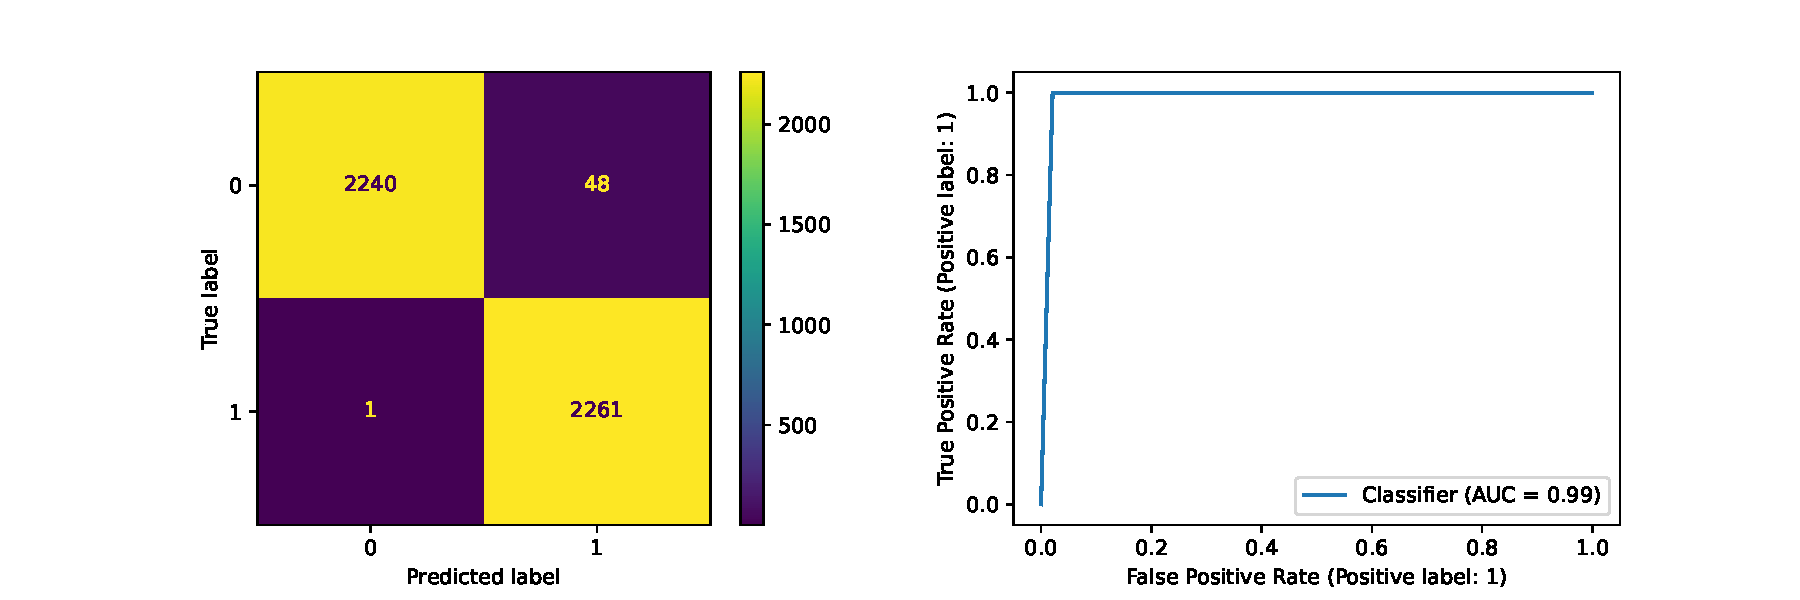
\includegraphics[scale=0.5]{tree}
\end{center}

Готовый классификатор \texttt{DecisionTreeClassifier} показывает схожие результаты.
\begin{lstlisting}[frame=none, numbers=none]
Accuracy: 0.9868131868131869
Precision: 0.9766233766233766
Recall: 0.9973474801061007
\end{lstlisting}
\begin{center}
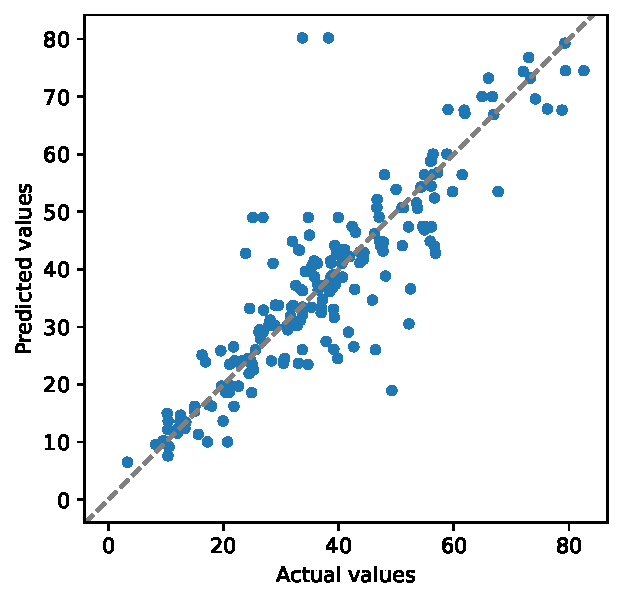
\includegraphics[scale=0.5]{sk_tree}
\end{center}
\pagebreak

Визуализируем разделющую поверхность решающего дерева.

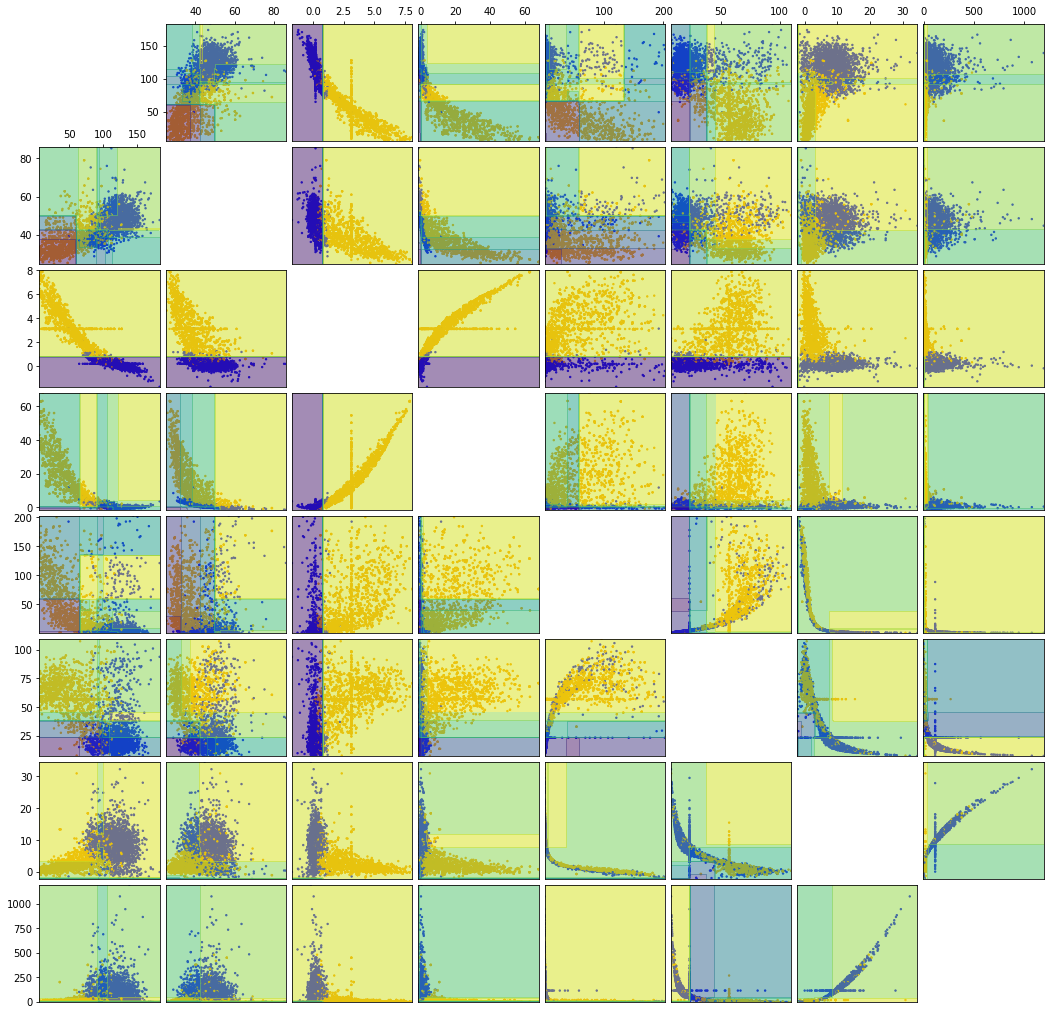
\includegraphics[width=\textwidth]{tree_boundaries}

Так как предсказания делаются всего по двум признакам, в узлах дерева с другими признаками ответ из обоих потомков усредняется. Поэтому это не отражает совсем полной картины разделения. Тем не менее, видно, что большая часть разделения происходит из-за признака, по которому классы очень хорошо разделяются одной точкой.
\pagebreak

\subsection*{Голосование}

Жесткое и мягкое госование реализовано в рамках одного класса. Мягкое госование усредняет предсказанные вероятности. Жесткое интрепретирует как вероятности долю моделей, предсказавших этот класс.

\begin{lstlisting}[language=python, keepspaces=true]
class Voting(BaseEstimator, ClassifierMixin):
    def __init__(self, estimators, mode='soft', pretrained=False):
        self.estimators = estimators
        self.mode = mode
        self.pretrained = pretrained
    
    def fit(self, data, labels):
        self.classes = len(np.unique(labels))
        if not self.pretrained:
            for estimator in self.estimators:
                estimator.fit(data, labels)
        return self
    
    def predict(self, data):
        return self.predict_proba(data).argmax(axis=1)
        
    def predict_proba(self, data):
        if self.mode == 'hard':
            pred = np.stack([est.predict(data) for est in self.estimators], axis=-1)
            res = np.zeros((len(data), self.classes))
            for i, p in enumerate(pred):
                v, c = np.unique(p, return_counts=True)
                res[i][v] += c
                res[i] /= len(self.estimators)
            return res
        else:
            pred = np.stack([est.predict_proba(data) for est in self.estimators], axis=1)
            return pred.mean(axis=1)
\end{lstlisting}
\pagebreak

Объединение KNN, байесовского классификатора, логистической регрессии, SVM и решающего дерева. Жесткое голосование.
\begin{lstlisting}[frame=none, numbers=none]
Accuracy: 0.9624175824175825
Precision: 0.9865053513261982
Recall: 0.9372236958443855
\end{lstlisting}
\begin{center}
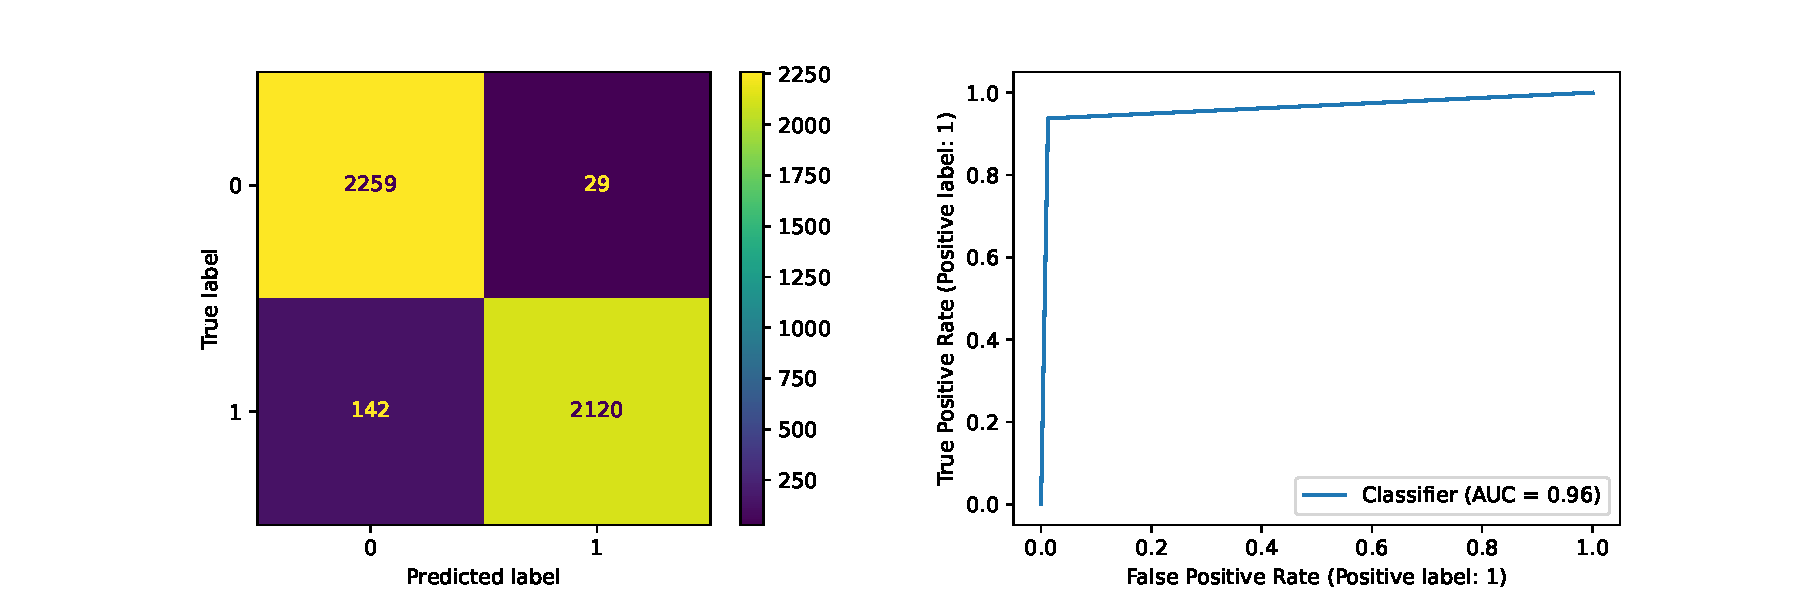
\includegraphics[scale=0.5]{all_hard}
\end{center}

Мягкое голосование.
\begin{lstlisting}[frame=none, numbers=none]
Accuracy: 0.9716483516483516
Precision: 0.9907961343764381
Recall: 0.9518125552608311
\end{lstlisting}
\begin{center}
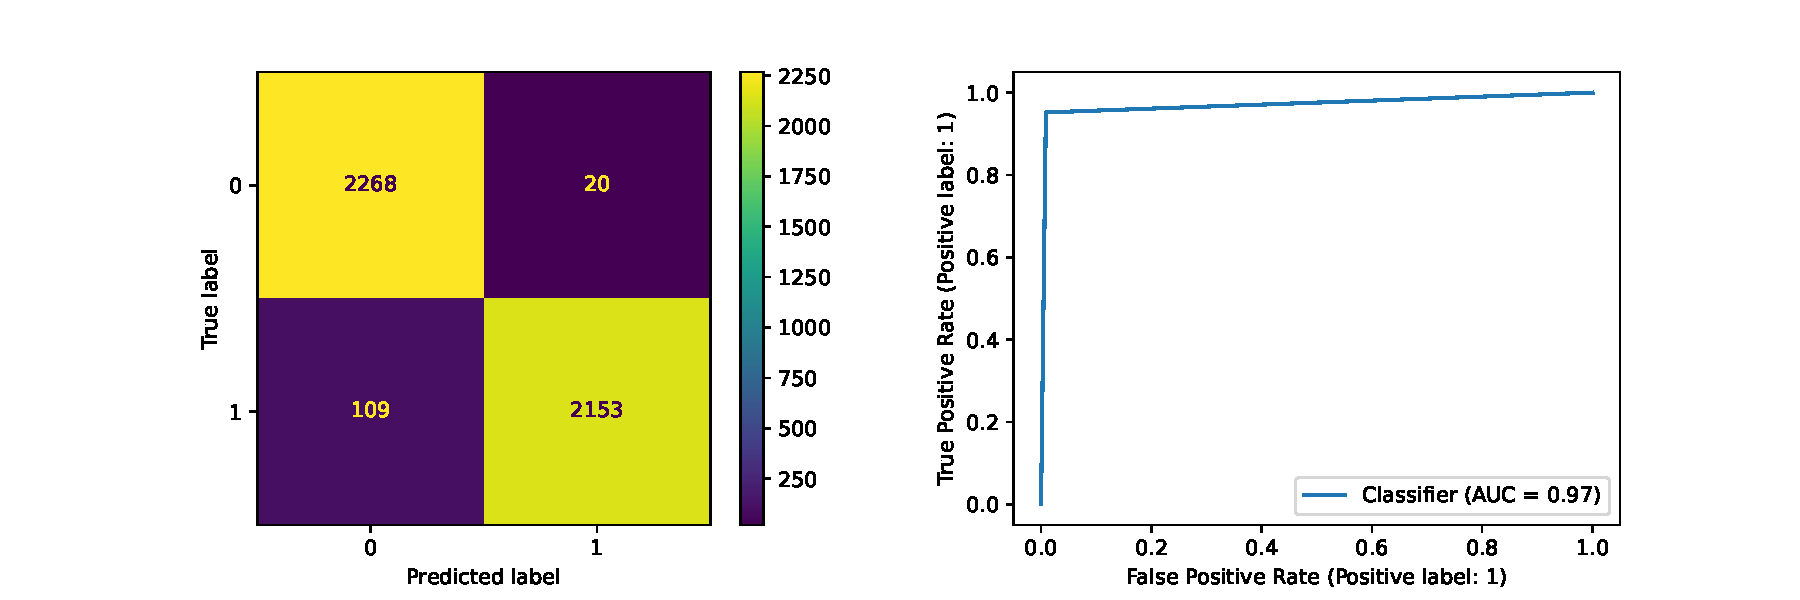
\includegraphics[scale=0.5]{all_soft}
\end{center}

Наилучшие результаты показывает мягкое объединение двух самых лучших классификаторов --- KNN и решающего дерева.
\begin{lstlisting}[frame=none, numbers=none]
Accuracy: 0.998021978021978
Precision: 0.996474217717056
Recall: 0.9995579133510168
\end{lstlisting}
\begin{center}
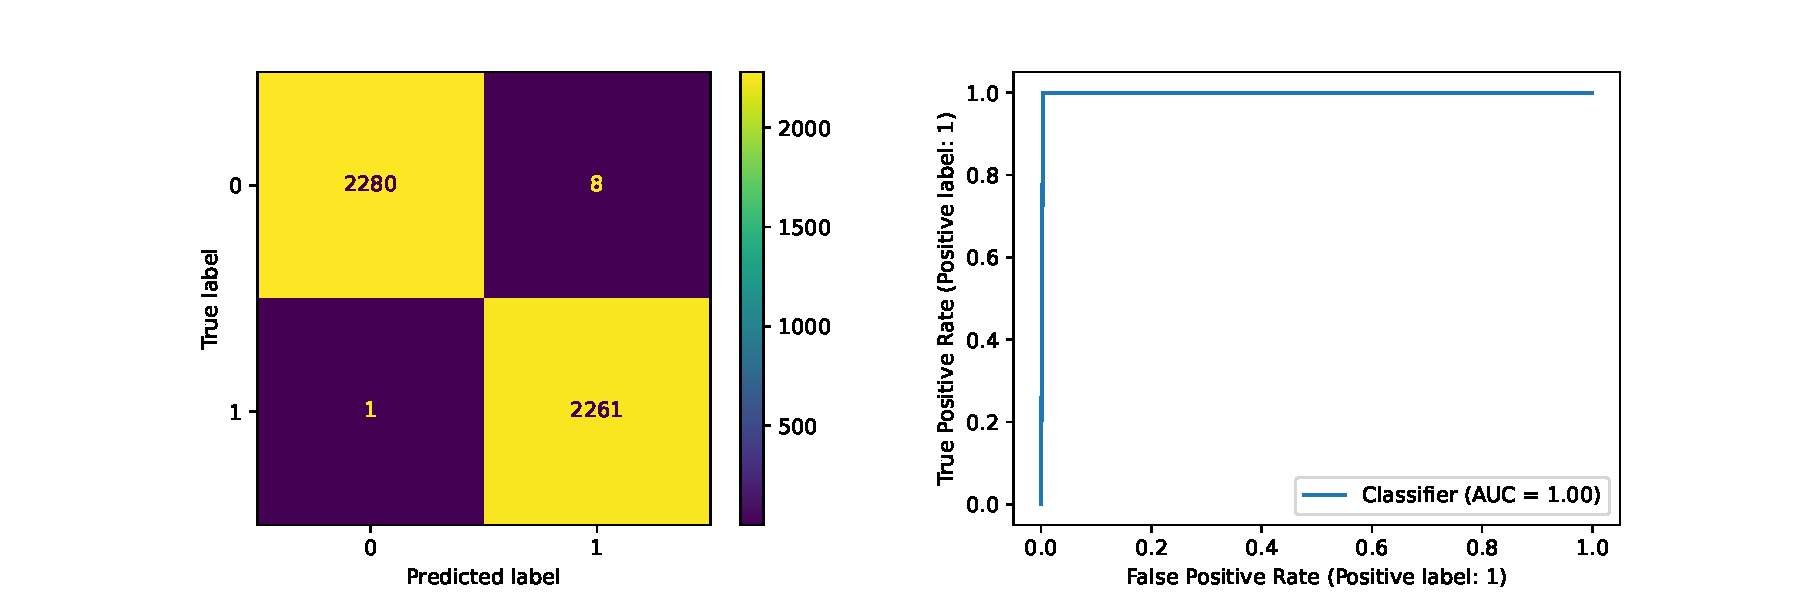
\includegraphics[scale=0.5]{two_best_soft}
\end{center}

\subsection*{Случайный лес}

Случайный лес использует множество решающих деревьев, каждое из которых обучается на случайной (с повторениями) подвыборке обучающих данных и подмножестве признаков. Предсказания деревьев объединяются по принципу мягкого голосования.

\begin{lstlisting}[language=python, keepspaces=true]
class RandomForest(BaseEstimator, ClassifierMixin):
    def __init__(self, n_estimators=100, min_leaf_size=5, max_depth=None, criterion=entropy, max_features='sqrt', max_samples=0.8):
        self.n_estimators = n_estimators
        self.min_leaf_size = min_leaf_size
        self.max_depth = max_depth
        self.criterion = criterion
        self.max_features = max_features
        self.max_samples = max_samples
        
    def fit(self, data, labels):
        features = np.arange(data.shape[1])
        indexes = np.arange(len(data))
        samples = math.floor(self.max_samples * len(data))
        if self.max_features == 'sqrt':
            max_features = math.floor(np.sqrt(len(features)))
        else:
            max_features = math.floor(len(features) * self.max_features)
        self.estimators = []
        for _ in range(self.n_estimators):
            np.random.shuffle(features)
            self.estimators.append(DecisionTree(min_leaf_size=self.min_leaf_size, max_depth=self.max_depth, criterion=self.criterion, features=features[:max_features]))
            idx = np.random.choice(indexes, (samples, ))
            self.estimators[-1].fit(data[idx], labels[idx])
        
    def predict_proba(self, data):
        pred = np.stack([est.predict_proba(data) for est in self.estimators], axis=1)
        return pred.mean(axis=1)
    
    def predict(self, data):
        return self.predict_proba(data).argmax(axis=1)
\end{lstlisting}

Результаты модели с 30 деревьями:

\begin{lstlisting}[frame=none, numbers=none]
Accuracy: 0.9973626373626374
Precision: 0.9947229551451188
Recall: 1.0
\end{lstlisting}
\begin{center}
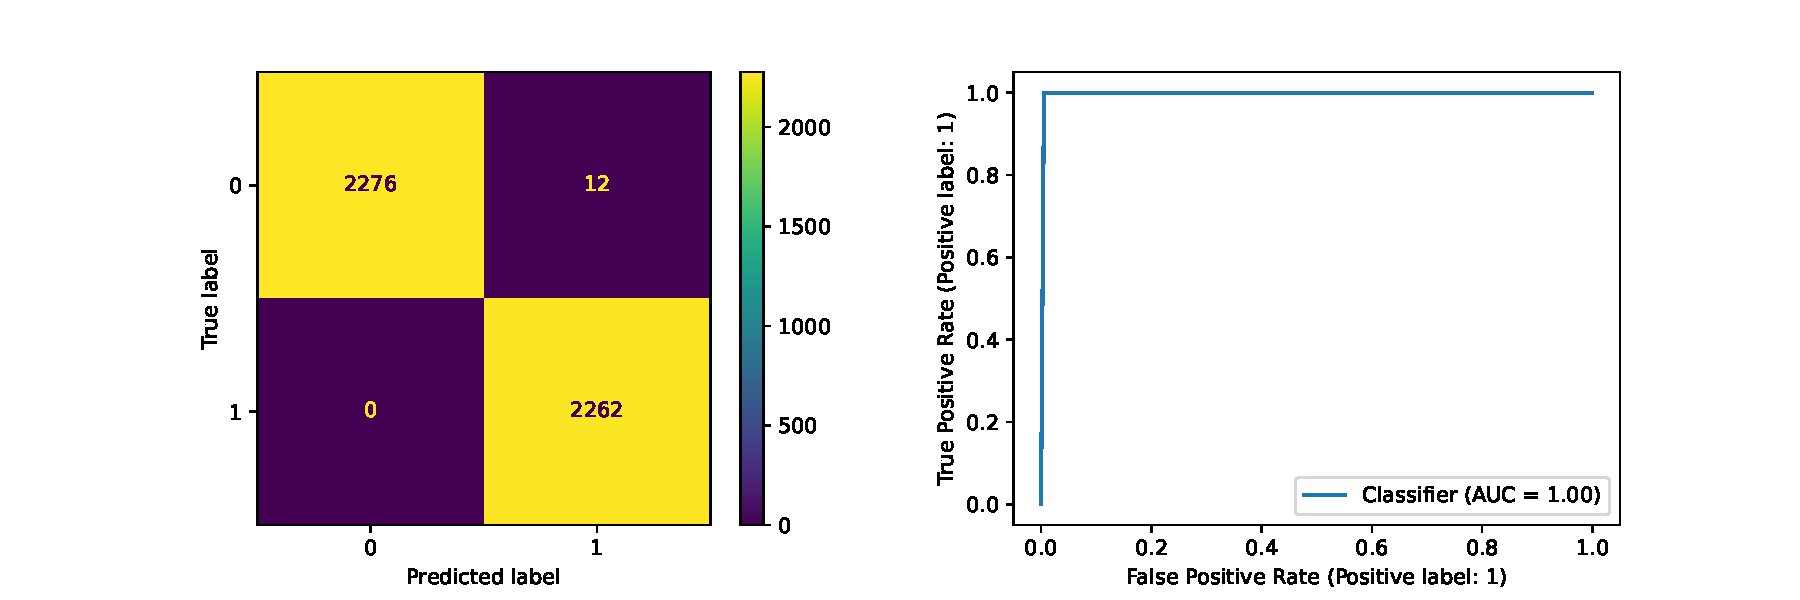
\includegraphics[scale=0.5]{random_forest}
\end{center}

\subsection*{Градиентный бустинг}

В качестве градиентного бустинга испытаны готовые реализации из библиотек \texttt{sklearn} и \texttt{catboost}.

\texttt{GradientBoostingClassifier:}
\begin{lstlisting}[frame=none, numbers=none]
Accuracy: 0.9958241758241758
Precision: 0.9916703200350724
Recall: 1.0
\end{lstlisting}
\begin{center}
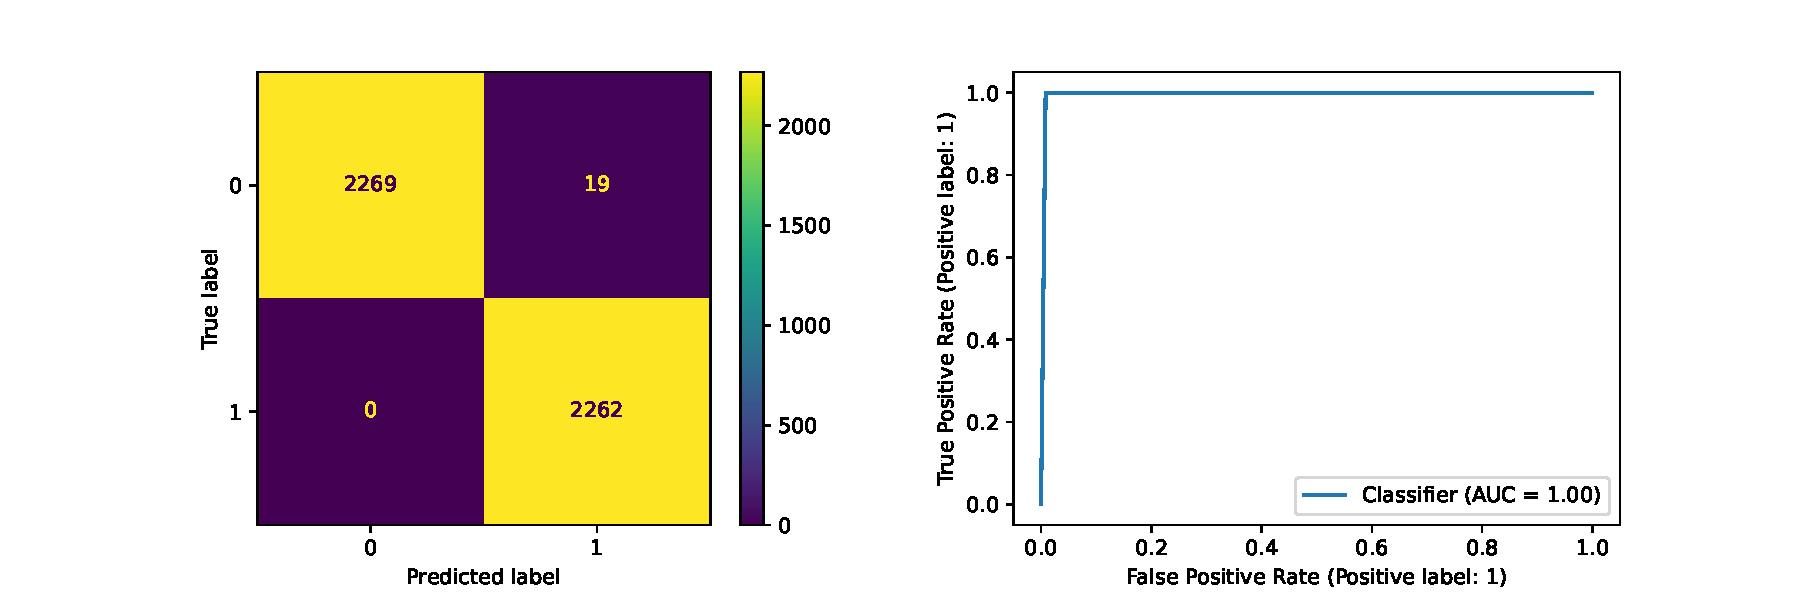
\includegraphics[scale=0.5]{grad_boost}
\end{center}

\texttt{CatBoostClassifier:}
\begin{lstlisting}[frame=none, numbers=none]
Accuracy: 0.9945054945054945
Precision: 0.9890686488850022
Recall: 1.0
\end{lstlisting}
\begin{center}
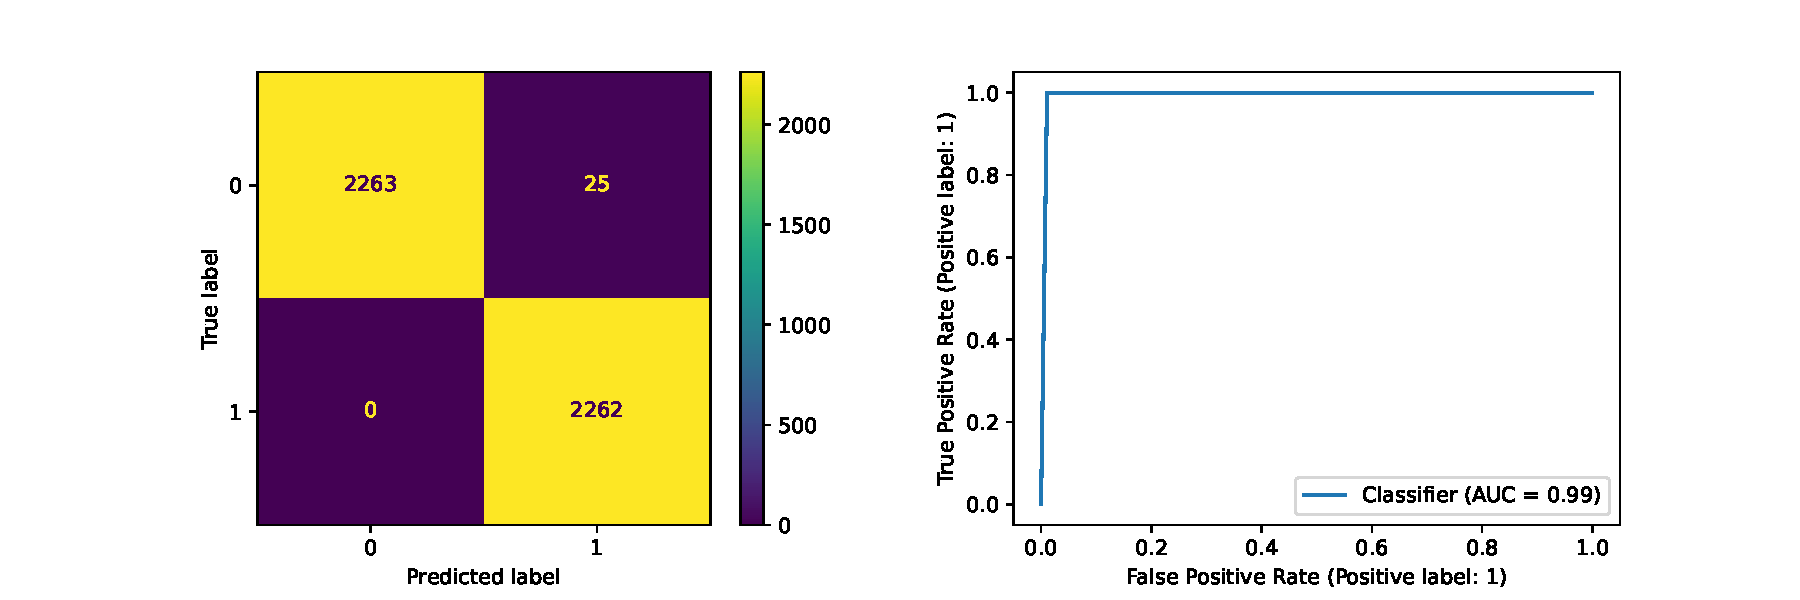
\includegraphics[scale=0.5]{cat_boost}
\end{center}

\pagebreak
